% -*- compile-command: "make jss-paper.pdf" -*-
\documentclass{article}

\usepackage{fullpage}
\newcommand{\R}{\proglang{R}}
% For algorithms
\usepackage{algorithm}
\usepackage{algorithmic}

% As of 2011, we use the hyperref package to produce hyperlinks in the
% resulting PDF.  If this breaks your system, please commend out the
% following usepackage line and replace \usepackage{icml2016} with
% \usepackage[nohyperref]{icml2016} above.
\usepackage{hyperref}
\usepackage{xcolor}
\definecolor{Ckt}{HTML}{E41A1C}
\definecolor{Min}{HTML}{4D4D4D}%grey30
%{B3B3B3}%grey70
\definecolor{MinMore}{HTML}{377EB8}
\definecolor{Data}{HTML}{984EA3}

% Packages hyperref and algorithmic misbehave sometimes.  We can fix
% this with the following command.
%\newcommand{\theHalgorithm}{\arabic{algorithm}}

% Employ the following version of the ``usepackage'' statement for
% submitting the draft version of the paper for review.  This will set
% the note in the first column to ``Under review.  Do not distribute.''
%\usepackage{icml2016} 
%\usepackage{fullpage}

% Employ this version of the ``usepackage'' statement after the paper has
% been accepted, when creating the final version.  This will set the
% note in the first column to ``Proceedings of the...''
%\usepackage[accepted]{icml2016}

\usepackage{tikz}
\usetikzlibrary{arrows}
\usepackage{amssymb,amsmath}
\usepackage{natbib}
\usepackage{amsthm}
\newtheorem{proposition}{Proposition}
\newtheorem{lemma}{Lemma}
\newtheorem{theorem}{Theorem}
\newtheorem{definition}{Definition}
\DeclareMathOperator*{\argmin}{arg\,min}
\DeclareMathOperator*{\sign}{sign}
\DeclareMathOperator*{\Lik}{Lik}
\DeclareMathOperator*{\Peaks}{Peaks}
\DeclareMathOperator*{\HotSpots}{HotSpots}
\newcommand{\Cost}{\text{Cost}}
\usepackage{stfloats}
\DeclareMathOperator*{\Diag}{Diag}
\DeclareMathOperator*{\TPR}{TPR}
\DeclareMathOperator*{\Segments}{Segments}
\DeclareMathOperator*{\Changes}{Changes}
\DeclareMathOperator*{\FPR}{FPR}
\DeclareMathOperator*{\argmax}{arg\,max}
\DeclareMathOperator*{\maximize}{maximize}
\DeclareMathOperator*{\minimize}{minimize}
\newcommand{\ZZ}{\mathbb Z}
\newcommand{\NN}{\mathbb N}
\newcommand{\RR}{\mathbb R}


%% -- LaTeX packages and custom commands ---------------------------------------

%% recommended packages
\usepackage{thumbpdf,lmodern}

%% another package (only for this demo article)
\usepackage{framed}

%% new custom commands
\newcommand{\class}[1]{`\code{#1}'}
\newcommand{\fct}[1]{\code{#1()}}


%% -- Article metainformation (author, title, ...) -----------------------------

%% - \author{} with primary affiliation
%% - \Plainauthor{} without affiliations
%% - Separate authors by \And or \AND (in \author) or by comma (in \Plainauthor).
%% - \AND starts a new line, \And does not.
\author{Toby Dylan Hocking}

%% - \title{} in title case
%% - \Plaintitle{} without LaTeX markup (if any)
%% - \Shorttitle{} with LaTeX markup (if any), used as running title
\title{A graph-constrained segmentation model for multi-modal
  regression, with application to peak summit detection in genomic
  data}

\begin{document}

\begin{figure}
  \centering
  \begin{minipage}{2in}
    \centering
    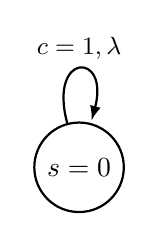
\begin{tikzpicture}[->,>=latex,shorten >=1pt,auto,node distance=2cm,
      thick,main node/.style={circle,draw}]

      \node[main node] (0) {$s=0$};

      \path[every node/.style={font=\sffamily\small}]
      (0) edge [loop above] node {$c=1,\lambda$} (0);
    \end{tikzpicture}
  \end{minipage}
  \begin{minipage}{2in}
    \centering
    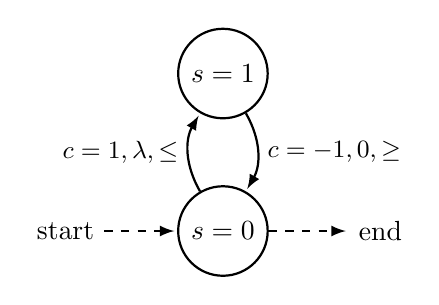
\begin{tikzpicture}[->,>=latex,shorten >=1pt,auto,node distance=2cm,
      thick,main node/.style={circle,draw}]

      \node[main node] (1) {$s=1$};
      \node[main node] (0) [below of=1] {$s=0$};
      \node (start) [left of=0] {start};
      \node (end) [right of=0] {end};

      \path[every node/.style={font=\sffamily\small}]
      (0) edge [bend left] node {$c=1, \lambda, \leq$} (1)
      (start) edge [dashed] (0)
      (0) edge [dashed] (end)
      (1) edge [bend left] node {$c=-1, 0, \geq$} (0);
    \end{tikzpicture}
  \end{minipage}
  \begin{minipage}{2in}
    \centering
    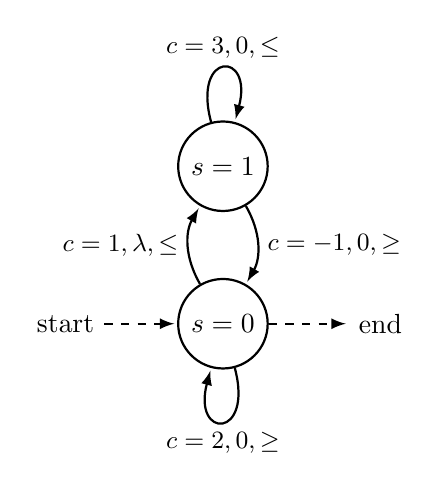
\begin{tikzpicture}[->,>=latex,shorten >=1pt,auto,node distance=2cm,
      thick,main node/.style={circle,draw}]

      \node[main node] (1) {$s=1$};
      \node[main node] (0) [below of=1] {$s=0$};
      \node (start) [left of=0] {start};
      \node (end) [right of=0] {end};

      \path[every node/.style={font=\sffamily\small}]
      (0) edge [bend left] node {$c=1, \lambda, \leq$} (1)
      (start) edge [dashed] (0)
      (0) edge [dashed] (end)
      (0) edge [loop below] node {$c=2,0,\geq$} (0)
      (1) edge [loop above] node {$c=3,0,\leq$} (1)
      (1) edge [bend left] node {$c=-1, 0, \geq$} (0);
    \end{tikzpicture}
  \end{minipage}
  \caption{State graphs for two changepoint models. Nodes represent
    states and solid edges represent changepoints. }
  \label{fig:state-graph}
\end{figure}

For genomic data such as ChIP-seq \citep{chip-seq}, it is desirable to
have a changepoint model which is interpretable in terms of peaks
(large values) and background noise (small values). We therefore
propose a model based on the graph shown in
Figure~\ref{fig:state-graph}. 

\begin{figure}
  \centering
  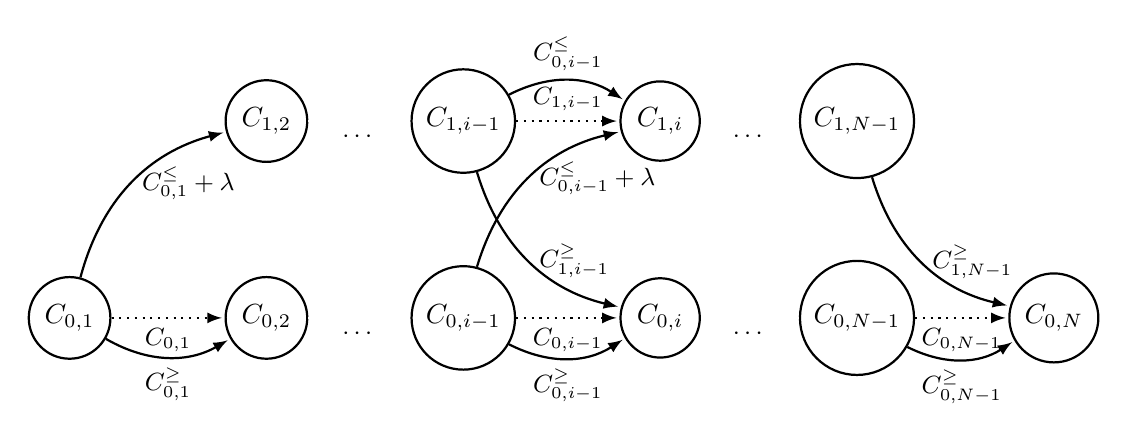
\begin{tikzpicture}[->,>=latex,shorten >=1pt,auto,node distance=2.5cm,
    thick,main node/.style={circle,draw}]
    \node[main node] (peak_t1) {$ C_{1,i-1}$};
    \node[main node] (bkg_t1) [below of=peak_t1] {$ C_{0,i-1}$};
    \node[main node] (peak_t) [right of=peak_t1] {$ C_{1,i}$};
    \node[main node] (bkg_t) [right of=bkg_t1] {$ C_{0,i}$};
    \node[main node] (peak_2) [left of=peak_t1] {$ C_{1,2}$};
    \node[main node] (bkg_2) [left of=bkg_t1] {$ C_{0,2}$};
    \node[main node] (peak_N1) [right of=peak_t] {$ C_{1,N-1}$};
    \node[main node] (bkg_N1) [right of=bkg_t] {$ C_{0,N-1}$};
    \node[main node] (bkg_N) [right of=bkg_N1] {$ C_{0,N}$};
    \node[main node] (bkg_1) [left of=bkg_2] {$ C_{0,1}$};
    \path[every node/.style={font=\small}]
    (peak_t1) edge [dotted] node {$ C_{1,i-1}$} (peak_t)
    (peak_t1) edge [black, bend right] node [right] {$ C_{1,i-1}^{\geq}$} (bkg_t)
    (bkg_t1) edge [dotted] node[midway, below] {$ C_{0,i-1}$} (bkg_t)
    (bkg_t1) edge [black, bend left] node[right] {$ C_{0,i-1}^{\leq}+\lambda$} (peak_t)
    (bkg_1) edge [black, bend left] node[right] {$ C_{0,1}^{\leq}+\lambda$} (peak_2)
    (bkg_1) edge [dotted] node[midway, below] {$ C_{0,1}$} (bkg_2)
    (peak_N1) edge [black, bend right] node [right] {$ C_{1,N-1}^{\geq}$} (bkg_N)
    (bkg_N1) edge [dotted] node[midway, below] {$ C_{0,N-1}$} (bkg_N)
    (bkg_2) edge [color=white] node[below, text=black, pos=0.5] {$\cdots$} (bkg_t1)
    (peak_2) edge [color=white] node[below, text=black, pos=0.5] {$\cdots$} (peak_t1)
    (bkg_N1) edge [color=white] node[below, text=black, pos=0.5] {$\cdots$} (bkg_t)
    (peak_N1) edge [color=white] node[below, text=black, pos=0.5] {$\cdots$} (peak_t)
    (bkg_1) edge [black, bend right] node[below] {$C_{0,1}^\geq$} (bkg_2)
    (bkg_N1) edge [black, bend right] node[below] {$C_{0,N-1}^\geq$} (bkg_N)
    (bkg_t1) edge [black, bend right] node[below] {$C_{0,i-1}^\geq$} (bkg_t)
    (peak_t1) edge [black, bend left] node[above] {$C_{0,i-1}^\leq$} (peak_t)
    ;
  \end{tikzpicture}
  \caption{Directed acyclic graph (DAG) representing dynamic
    programming computations (Algorithm~\ref{algo:GFPOP}) for
    changepoint model with up-down constraints between adjacent
    segment means. Nodes in the graph repesent cost functions, and
    edges represent inputs to the the MinOfTwo sub-routine
    (solid=changepoint, dotted=no change). There is one column for
    each data point and one row for each state: the optimal cost of
    the peak state $s=1$ at data point $i$ is $ C_{1,i}$ (top
    row); the optimal cost of the background noise state $s=0$ is
    $ C_{0,i}$ (bottom row). There is only one edge going to
    $ C_{0,2}$ and $ C_{1,2}$ because the model is
    constrained to start in the background noise state ($s_1=0$).}
  \label{fig:computation-graph}
\end{figure}

\includegraphics[width=\textwidth]{figure-Mono27ac-label-error}

\bibliographystyle{abbrvnat}
\bibliography{refs}

\end{document}
